% !TeX document-id = {f19fb972-db1f-447e-9d78-531139c30778}
% !BIB program = biber
\documentclass[compress]{beamer}
\usepackage[T1]{fontenc}
\usepackage{pifont}
\usetheme[block=fill,subsectionpage=progressbar,sectionpage=progressbar]{metropolis} 

\usepackage{wasysym}
\usepackage{etoolbox}
\usepackage[utf8]{inputenc}

\usepackage{threeparttable}
\usepackage{subcaption}

\usepackage{tikz-qtree}
\setbeamercovered{still covered={\opaqueness<1->{5}},again covered={\opaqueness<1->{100}}}


\usepackage{listings}

\lstset{
	basicstyle=\scriptsize\ttfamily,
	columns=flexible,
	breaklines=true,
	numbers=left,
	%stepsize=1,
	numberstyle=\tiny,
	backgroundcolor=\color[rgb]{0.85,0.90,1}
}



\lstnewenvironment{lstlistingoutput}{\lstset{basicstyle=\footnotesize\ttfamily,
		columns=flexible,
		breaklines=true,
		numbers=left,
		%stepsize=1,
		numberstyle=\tiny,
		backgroundcolor=\color[rgb]{.7,.7,.7}}}{}


\lstnewenvironment{lstlistingoutputtiny}{\lstset{basicstyle=\tiny\ttfamily,
		columns=flexible,
		breaklines=true,
		numbers=left,
		%stepsize=1,
		numberstyle=\tiny,
		backgroundcolor=\color[rgb]{.7,.7,.7}}}{}



\usepackage[american]{babel}
\usepackage{csquotes}
\usepackage[style=apa, backend = biber]{biblatex}
\DeclareLanguageMapping{american}{american-UoN}
\addbibresource{../../bdaca.bib}
\renewcommand*{\bibfont}{\tiny}

\usepackage{tikz}
\usetikzlibrary{shapes,arrows,matrix}
\usepackage{multicol}

\usepackage{subcaption}

\usepackage{booktabs}
\usepackage{graphicx}

\graphicspath{{../../pictures/}}

\makeatletter
\setbeamertemplate{headline}{%
	\begin{beamercolorbox}[colsep=1.5pt]{upper separation line head}
	\end{beamercolorbox}
	\begin{beamercolorbox}{section in head/foot}
		\vskip2pt\insertnavigation{\paperwidth}\vskip2pt
	\end{beamercolorbox}%
	\begin{beamercolorbox}[colsep=1.5pt]{lower separation line head}
	\end{beamercolorbox}
}
\makeatother



\setbeamercolor{section in head/foot}{fg=normal text.bg, bg=structure.fg}



\newcommand{\question}[1]{
	\begin{frame}[plain]
		\begin{columns}
			\column{.3\textwidth}
			\makebox[\columnwidth]{
				\includegraphics[width=\columnwidth,height=\paperheight,keepaspectratio]{mannetje.png}}
			\column{.7\textwidth}
			\large
			\textcolor{orange}{\textbf{\emph{#1}}}
		\end{columns}
\end{frame}}




\title[Big Data and Automated Content Analysis]{\textbf{Big Data \& Automated Content Analysis} \\ Week 10 -- Wednesday: »Supervised Approaches to Text Analysis II«}
\author[Damian Trilling]{Damian Trilling \\ ~ \\ \footnotesize{d.c.trilling@uva.nl \\@damian0604} \\ \url{www.damiantrilling.net}}
\date{14 April 2021}
\institute[UvA]{Afdeling Communicatiewetenschap \\Universiteit van Amsterdam}

\begin{document}
	
	\begin{frame}{}
		\titlepage
	\end{frame}
	
	\begin{frame}{Today}
		\tableofcontents
	\end{frame}


\begin{frame}[standout]
Also re-read chapter 8.5!
\end{frame}

\question{Everything clear from last week?}

\section{The problem of overfitting}


\question{Isn't training multiple models and then selecting the best one a bit like $p$-hacking?}


\begin{frame}{Yes. We call this problem ``overfitting''.}

\begin{figure}
	\centering
	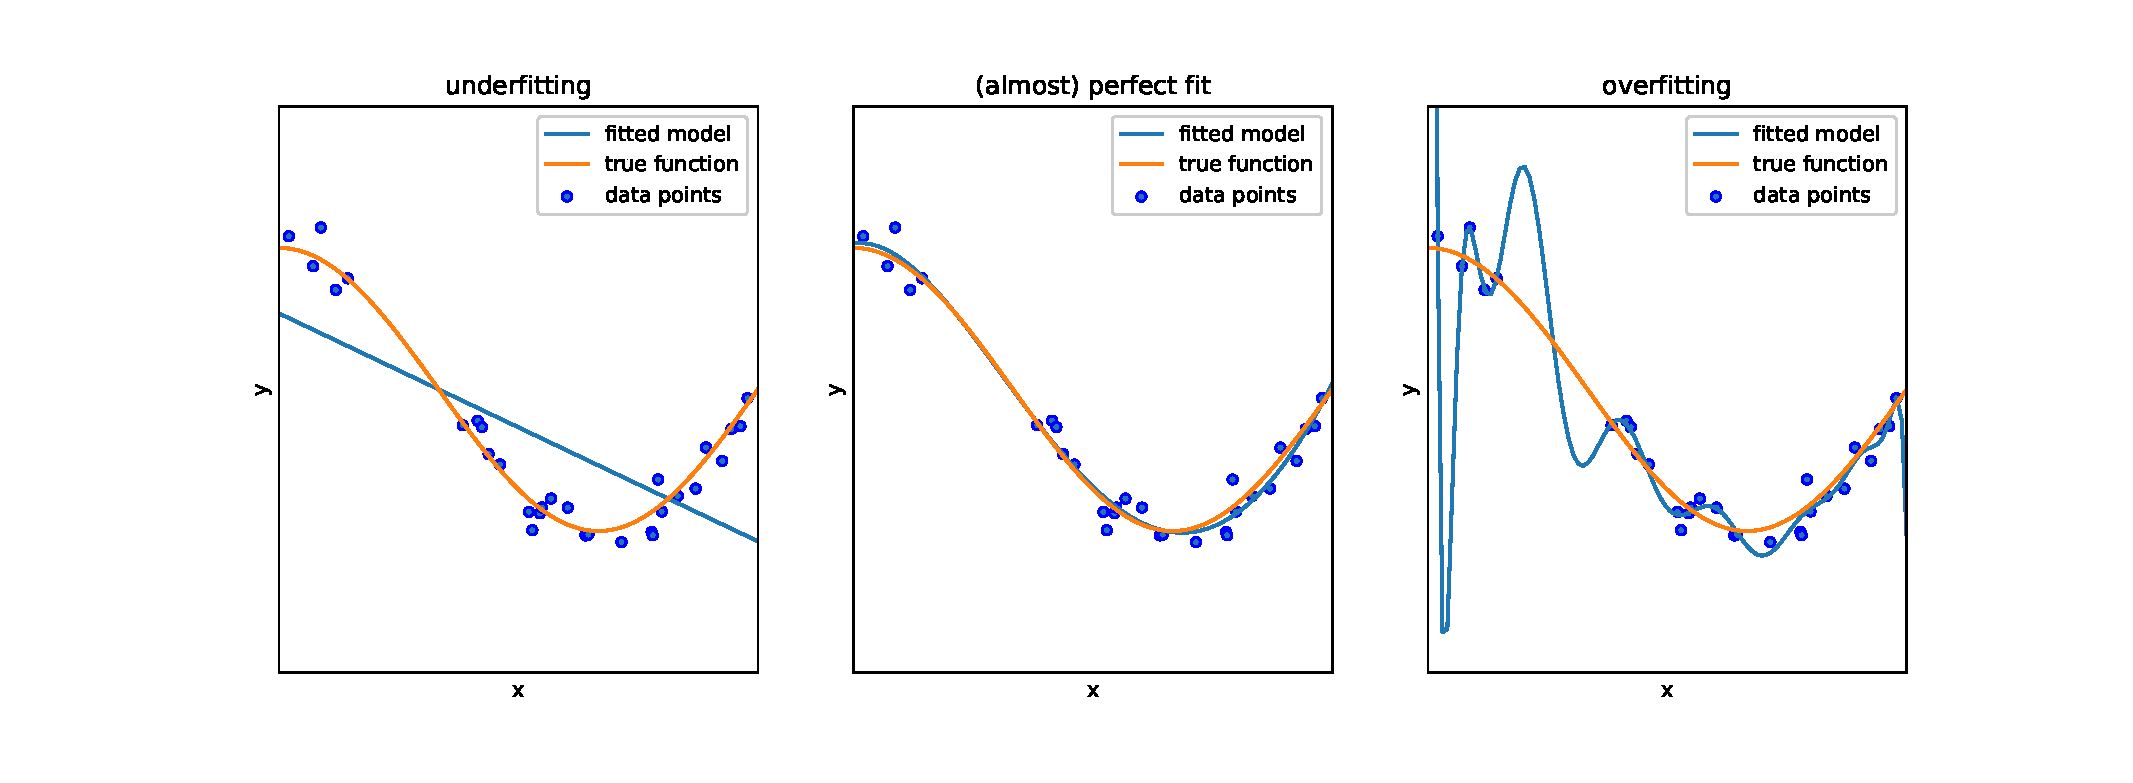
\includegraphics[width=\linewidth]{ch09_overfitting}
	\caption{Underfitting and overfitting. Example adapted from https://scikit-learn.org/stable/auto\_examples/model\_selection/plot\_underfitting\_overfitting.html}
	\label{fig:overfit}
\end{figure}
\end{frame}


\begin{frame}{How to avoid overfitting}
\begin{enumerate}[<+->]
	\item \textbf{Train/test split. } We already do this. It avoids overfitting on the training data.\footnote{In classical statistics, the $R^2$ of an OLS regression is prone to that. Calculating $R^2$ on a separate test set would be much more conservative.}
	\item \textbf{Train/validation/test split.} But maybe we overfit on the test data now? We could set aside \textit{third} dataset.
	\item \textbf{$k$-fold crossvalidation.} Extending the above such that every case is sometimes $k-1$ times part of the training data and 1 time part of the validation data.
	\item \textbf{Regularization.} (in combination with the above) We ``penalize'' models for being too complex.
\end{enumerate}

\end{frame}



\subsection{Train/validation/test split}

\begin{frame}{Train/validation/test split}
\begin{itemize}
	\item When you compare a lot of different models (or (hyper-)parameters), you might want to evaluate (compare) them using a third dataset 
	\item e.g., make 80/20 split (train/test); then split first part again 80/20 (train/validation)
	\item only use the test data \emph{at the very end} to get a final estimate of how good your model is.
\end{itemize}
\pause
In short: Validation data to \emph{select} the best approach; test data to get the accuracy of the approach you chose.
\end{frame}

\subsection{Cross-validation}



\begin{frame}[plain]
	
	\begin{figure}
		\centering
		\includegraphics[width=.8\linewidth]{gridsearchcrossvalidation}
		\caption{First, we set aside a test dataset for the final evaluation. Then, we split our data into $k=5$ folds, where each fold is used for validation once (blue) and $k-1=4$ times for training.
			\tiny Source: \url{https://scikit-learn.org/stable/_images/grid_search_cross_validation.png}}
		\label{fig:crossval}
	\end{figure}
\end{frame}



\begin{frame}[fragile]{Cross-validation}
\begin{lstlisting}
from sklearn.model_selection import cross_val_score
from sklearn.naive_bayes import MultinomialNB
nb = MultinomialNB()     # the classifier we trained last week
scores = cross_val_score(nb,  train_features, [r[1] for r in reviews], cv=10)
print(scores)
\end{lstlisting}

results in:

\begin{lstlisting}
[0.858  0.8612 0.8516 0.8528 0.8672 0.8664 0.8576 0.8652 0.8436 0.852 ]
\end{lstlisting}

We estimate the model 10 times on different trainig/validation data splits and get 10 different evaluation scores (here: accuracy, but we can use precision, recall, F1, etc. -- see examples in the book).

Note that a simple 50:50 train/validation split is identical to setting $k=2$ 

{\tiny See for more info
	\url{https://scikit-learn.org/stable/modules/cross\_validation.html}}
\end{frame}



\begin{frame}{Reasons to do Cross-validation}
	\begin{block}{We can get confidence intervals around the scores}
		\begin{itemize}
			\item If we have 10 scores instead of one, we can not only get the mean, but also a standarddeviation
			\item If you have two models, both with a mean accuracy (or F1, or whatever) of .85 but one with a large and one with a low standard deviation, you probably prefer the latter -- it generalizes better, less likely to suffer from overfitting
		\end{itemize}	
	\end{block}

\end{frame}






\begin{frame}{Reasons to do Cross-validation}
	\begin{block}{We do not ``waste'' too much validation data}
		\begin{itemize}
			\item If $k=10$ (the most typical value), in each iteration, we use 90\% of the data for training.
			\item We even use \emph{all} data (except test set, of course) for training at least once.
			\item With train/validation split, we probably need a larger validation set to be sure (e.g., 80/30)
			\item Especially relevant when annotation is expensive.
		\end{itemize}
	\end{block}
\end{frame}



\begin{frame}[allowframebreaks]{Takeaway}

\begin{block}{Simple train/test split}
\begin{itemize}
	\item introductory examples/pedagical reasons
	\item really small dataset where you cannot afford to set aside validation data
	\item if -- for whatever reason -- you do not compare different models and settings.
\end{itemize}
\end{block}

\framebreak

\begin{block}{Train/validation/test split}
	\begin{itemize}
		\item To compare different model configurations without overfitting on the test data
		\item Pedacogical reasons, simple start
		\item Very large datasets or very complex models where setting $k>2$ would lead to prohibtitively expensive computations
	\end{itemize}
\end{block}

\framebreak

\begin{block}{$k$-fold crossvalidation}
	\begin{itemize}
		\item Best option for comparing multiple models, \emph{especially} when engaging in \emph{hyperaparameter tuning} (next section)
	\end{itemize}
\end{block}

\pause
\begin{alertblock}{Also a nice example for changing standards in the field}
A couple of years ago, you could get away with just doing a train/test split in your paper. Nowadays, chances are high a reviewer will reject this (if you try to publish your Master's thesis, for instance).
\end{alertblock}


\end{frame}



\begin{frame}[standout]
In other words: wether you have or create a train/validation/test or use cross-validation -- just make sure you always set aside one test set for final evaluation that you have never used before.
\end{frame}





\section{Finding the optimal (hyper-)parameters}

\begin{frame}[plain]
\centering
	\begin{description}
		\item[\textcolor{red}{hyperparameter}] a parameter of a model that is not learned through training, but specified in advance
	\end{description}
	
\end{frame}



\subsection{Grid search}

\begin{frame}{Hyperparameter optimization with grid search}
\begin{block}{General idea}
	Rather than arbitrary trying some configurations, let's systematically test and compare.
\end{block}
First idea: Use a for-loop! (Example 11.4 in the book)
\end{frame}

\begin{frame}[plain,fragile]
	\small
\begin{lstlisting}
configurations = 
[('NB with Count', CountVectorizer(min_df=5, max_df=.5), MultinomialNB()),
('NB with TfIdf', TfidfVectorizer(min_df=5, max_df=.5), MultinomialNB()),
('LogReg with Count', CountVectorizer(min_df=5, max_df=.5), LogisticRegression(solver='liblinear')),
('LogReg with TfIdf', TfidfVectorizer(min_df=5, max_df=.5), LogisticRegression(solver='liblinear'))]

for description, vectorizer, classifier in configurations:
    print(description)
    X_train = vectorizer.fit_transform(reviews_train)
    X_test = vectorizer.transform(reviews_test)
    classifier.fit(X_train, y_train)
    y_pred = classifier.predict(X_test)
    short_classification_report(y_test, y_pred)
    print('\n')
\end{lstlisting}
(where (X\_test, y\_test) hopefully refers to a validation dataset with another test dataset set aside) 
\end{frame}


\begin{frame}{A wishlist}
We now tested $2\times 2$ combinations: (NB|LogReg) $\times$ (count|tf$\cdot$ idf).

	Wouldn't it be nice if we\ldots
\begin{itemize}[<+->]
	\item could simply state this instead of manually creating the list?
	\item (especially if we had  (NB|LogReg) $\times$ (count|tf$\cdot$ idf)  $\times$ (min\_df=5|min\_df=1)  $\times$ (max\_df=.5|max\_df=.8 |max\_df=.9)  $= 2\times 2\times 2\times 3 = 24$ options)
	\item would not have to check manually which one performed best?
\end{itemize}
\pause
\textbf{That's what scikit-learn's gridsearch functionality does!} (and the second bullet point is called the \textit{grid})
\end{frame}


\begin{frame}[standout]
Gridsearch is especially useful for \textcolor{orange}{hyperparameter optimization}, such as trying out different values for min\_df and max\_df on the previous slide.

You could also use a combined approach where you first use a handwritten loop to narrow down the number of candidate models and then tune the model(s) you settled on with a grid search.
\end{frame}


\subsection{A typical case for gridsearch: The regularization parameter C}


\begin{frame}{The regularization parameter $\lambda$ (or $C = .5n\lambda$)}
$$
%\underset{\boldsymbol{\beta}}{\arg \min }\left[\sum_{i=1}^{n}\left(Y_{i}-\beta_{0}-\sum_{j=1}^{p} \beta_{j} X_{j i}\right)^{2}+\lambda \sum_{j=1}^{p}\left|\beta_{j}\right|^{q}\right]
\underset{\boldsymbol{\beta}}{\arg \min }\left[\color{blue} \sum_{i=1}^{n}\left(Y_{i}-\beta_{0}-\sum_{j=1}^{p} \beta_{j} X_{j i}\right)^{2}\color{orange} +\lambda \sum_{j=1}^{p}\left|\beta_{j}\right|^{q} \color{black} \right]
$$

\color{blue}We estimate the $\beta$-coefficients of a model by optimizing a so-called loss function, i.e minimizing the ``cost'' that occurs when the prediction is wrong.

\color{orange} \emph{If we simply add the sum of the $\beta$ coefficients} to the model, we ``punish'' large coefficients.
\color{black}
\pause

If $\lambda$ is larger, we punish more.

\tiny{If $q=1$, we call it L1 regularization. If we add the squared coefficients ($q=2$), we call it L2 regularization.}
\end{frame}



\begin{frame}{The regularization parameter $\lambda$ (or $C = .5n\lambda$)}
\begin{itemize}[<+->]
	\item scikit-learn uses regularization by default
	\item (that's why the coefficients of a logistic regression classifier will differ from a ``tradtional'' logistic regression with the statsmodels module)
	\item Remember that we are \textit{not} interested in a substantive interpretation of the  $\beta$-coefficients but in a good prediction (which is why ``punishing'' large coefficients and hence biasing the coeffients is not a problem at all!)
	\item The penalty will shrink the coefficients towards zero, \emph{which is very useful to avoid overfitting!}
	\item As always, there is a lot of extra info on the scikit-learn website
\end{itemize}
\end{frame}

\question{How harsh should the penalty be?}



\begin{frame}{Hyperparameter optimization with grid search}
	\begin{block}{General idea}
		Rather than arbitrary trying some combinations of hyperparameters, let's systematically test and compare.
	\end{block}
	
	\pause
	
	\begin{example}
		\begin{itemize}[<+->]
			\item To avoid overfitting, scikit-learn adds a \emph{regularization term} to the loss function that is minimized to fit the regression.
			\item Think of this term as a penalty for overfitting
			\item How much weight should our penalty carry? That's determined by a constant, $C$.
			\item How to determine the best $C$? $\Rightarrow$ grid search 
		\end{itemize}
	\end{example}
\end{frame}




\begin{frame}[fragile]{Hyperparameter optimization with grid search}
Finding $C$ in a logistic regression using 5-fold cross-validation
\begin{lstlisting}
from sklearn.linear_model import LogisticRegressionCV
logregCV = LogisticRegressionCV(cv=5).fit(train_features, [r[1] for r in reviews])
\end{lstlisting}
\pause 

\begin{itemize}[<+->]
	\item Here, we just need to use \texttt{LogisticRegressionCV} instead of \texttt{LogisticRegression}. 
	\item But we can use it to test any combination of choices
\end{itemize}
\end{frame}




\begin{frame}[plain,fragile]
	\small
\begin{lstlisting}
pipeline = Pipeline(steps = [('vectorizer', TfidfVectorizer()), ('classifier', LogisticRegression(solver='liblinear'))])
grid = {
    'vectorizer__ngram_range' : [(1,1), (1,2)],
    'vectorizer__max_df': [0.5, 1.0],
    'vectorizer__min_df': [0, 5],
    'classifier__C': [0.01, 1, 100]
}

search = GridSearchCV(estimator=pipeline,
                      param_grid=grid,
                      scoring='accuracy', 
                      cv=5,
                      n_jobs=-1,  # use all cpus
                      verbose=10)
search.fit(reviews_train, y_train)
print(f'Using these hyperparameters {search.best_params_}, we get the best performance:')
print(short_classification_report(y_test, search.predict(reviews_test)))
\end{lstlisting}
Example 11.6 (book)
\end{frame}

\begin{frame}[standout]
Note that the grid is specified as a dictionary where the keys are strings with the name of the step in the pipeline followed by two underscores followed by the parameter to tune, and the values are lists of values.

This means that \emph{any} parameter that the classifier or vectorizer takes can be tuned!
\end{frame}



\begin{frame}{The pipeline notation in scikit learn}
You might have notived the Pipeline construct in the last example.
	\begin{itemize}
		\item Machine learning involves multiple steps (e.g., preprocessing $\rightarrow$ vectorizer $\rightarrow$ classification)
		\item We did all of them seperately before
		\item Nothing wrong with that, but to ease use and evaluation \emph{of the whole process} (as needed for the gridsearch), we can define a \texttt{pipeline}.
	\end{itemize}
	
\end{frame}

\begin{frame}[fragile]{Let's rewrite our example from last week's slides as pipeline (and add cross-validation)}
\begin{lstlisting}
from sklearn.feature_extraction.text import TfidfVectorizer
from sklearn.linear_model import LogisticRegressionCV
from sklearn.pipeline import make_pipeline

vec = TfidfVectorizer()
clf = LogisticRegressionCV()
pipe = make_pipeline(vec, clf)

pipe.fit([r[0] for r in reviews], [r[1] for r in reviews])
predictions = pipe.predict([r[0] for r in test])
\end{lstlisting}
\end{frame}

\begin{frame}{Pipeline takeaway}
	\begin{itemize}
		\item In principle, just a different way to write what we already did
		\item The more steps, the more relevant (e.g., preprocessing $\rightarrow$ vectorizer $\rightarrow$ dimensionality-reduction $\rightarrow$ classification)
		\item The more you rely on automated evaluation (e.g., grid search) of \emph{multiple} steps in the pipeline, the more useful it is
	\end{itemize}
\end{frame}




\begin{frame}{Grid-search takeaway}
\begin{itemize}[<+->]
	\item When you want to systematically test what happens when you vary a hyperparameter, use grid-search to automatically do so and select the best value
	\item sometimes already implemented (e.g., \texttt{LogisticRegressionCV} as direct replacement for \texttt{LogisticRegression})
	\item But \texttt{GridSearchCV} is very flexible: can be used in combination with pipeline (wait a minute\ldots) for very different purposes
\end{itemize}


\end{frame}











\section[More suggestions ]{More suggestions for improving your models}



\subsection{Tuning decision thresholds with ROC curves}

\begin{frame}{From estimate to label}
\makebox[\linewidth]{\includegraphics[width=.5\paperwidth,height=\paperheight,keepaspectratio]{../../pictures/sigmoid}}
In logistic regression, we use the \textit{sigmoid function} to transform the estimates into probabilities.

To transform the probabilities into binary labels, we use a cutoff (default: 0.5).
\end{frame}

\begin{frame}{Why use 0.5 as cutoff?}
\begin{itemize}[<+->]
	\item It makes most sense (intuitively, mathematically)
	\item But remember our precision/recall tradeoff: maybe we want to be `stricter' or `less strict'
	\item Maybe it is importance to us that our classifier is balanced and equally good in predicting both classes, even if overall accuracy suffers (slightly) 
\end{itemize}
\pause
Let's see what happens if we plot False Positives against True Positives (ROC-curve)
\end{frame}


\begin{frame}{ROC Curve}
\makebox[\linewidth]{\includegraphics[width=.5\paperwidth,height=.5\paperheight,keepaspectratio]{../../pictures/roccurve}}
\begin{itemize}
	\item If we choose a threshold such that we get very little false positives, we also get too little true positives.
	\item Optimum in the upper left corner
\end{itemize}

\end{frame}


\begin{frame}{So, how to we determine the exact value? }
See notebook

\url{https://github.com/damian0604/bdaca/blob/master/12ec/week10/Determining\%20the\%20cutoff-point\%20in\%20logistic\%20regression.ipynb}
\end{frame}









\begin{frame}{Some further ideas to look into}

\begin{block}{Balancing classes}
Your classifier probably works better if you have approximately the same amount of annotated training data for both classes (e.g., pos/neg). If getting such data is not an option, you may consider weighing accordingly, e.g. using

\texttt{LogisticRegression(class\_weight='balanced')}
\end{block}

\end{frame}

\begin{frame}{Some further ideas to look into}

\begin{block}{More advanced pipelines}
	Consider constructing advanced pipelines, including a dimension reduction step: 
	
	
	\url{https://scikit-learn.org/stable/tutorial/statistical\_inference/putting\_together.html}
\end{block}

\end{frame}



\begin{frame}{Some further ideas to look into}

\begin{block}{Combine different feature sets}
	E.g, use BOW-features as well as features such as sentence length, number of sentences (or whatever)
	
	
	\url{
		https://scikit-learn.org/stable/auto\_examples/hetero\_feature\_union.html}
\end{block}




\end{frame}




\section{Next meetings}


\question{Any questions?}

\begin{frame}{Friday}

	\begin{itemize}
		\item Try it yourself! Ideally, on own data! (can also be via Google Dataset Search, Kaggle, \ldots)
		\item We are now at the point in the course where the Friday sessions move a bit away from specific instructions towards more freedom to work on your own data and projects.
\end{itemize}
Learning goals: 
\begin{itemize}
		\item Apply techniques to new datasets. 
		\item Be able to construct the whole pipeline from ingesting via preprocessing to final prediction
	\end{itemize}
	
\end{frame}

\begin{frame}{Take-home exam week 11}
\begin{itemize}
	\item Again, three tasks: literature, programming, advice
	\item Main focus: Machine Learning
\end{itemize}
\end{frame}


%\begin{frame}[plain,allowframebreaks]
%	\printbibliography
%\end{frame}


\end{document}

